\chapter{Results and Analysis}
\section{Evaluation setup}
Two experiments were run with an identical design, one on the reference transformer and one on Qwen2.5-0.5B-Instruct. Each experiment is a full factorial grid of three memory arms (shared KV, text only, isolated), nine semantic-pressure levels ($\pi = 0, 0.125, \dots, 1$, that is, 0 to 16 one-sided statements out of 16) and five seeds, giving 135 two-agent conversations per model and 270 in total. Every conversation has four rounds (eight turns), the sender reads four statements per round, and each reply is limited to ten tokens. The five seeds select the probe and the order of statements; with the fixed master seed of the probe bank they draw four distinct fictional groups, one in each bias category (gender, religion, disability and socio-economic status), with the religion probe drawn twice under different seeds. The reference experiment ran on the laptop CPU and the Qwen2.5 experiment on the GTX 1650~Ti GPU in 32-bit precision; the hardware and software are listed in Tables~\ref{tab:hw} and~\ref{tab:sw}.

Several safeguards protect the comparisons from bias and invalid conclusions. All thresholds, corrections, controls and the coherence budget (Table~\ref{tab:thresholds}) were fixed before the main runs. Both caches are seeded identically in every arm, and the same seed produces the same statements in every arm, so the arms differ only in the channel between the agents. Interventions are evaluated by seed-matched replay, so an intervened run differs from its baseline only in the edit, and against two negative controls. Attention sinks are held out from the attractor class. Group names are fictional, so the bias measured in a conversation is caused by that conversation rather than by the model's prior beliefs about a real group. The only adaptive step was the one foreseen in the design workflow: when no intervention on the first target set was accepted, a second, refined target set was tried, and both attempts are reported below. Finally, the reference experiment was re-run from scratch at the end of the project and reproduced every reported value.

\section{Evaluation criteria}
Table~\ref{tab:criteria} lists the criteria used to assess each objective. The primary behavioural measure is the bias index $B \in [-1, 1]$ of Section~5.2.4, reported where helpful as the probability $(1+B)/2$ of choosing the stereotype trait. Contagion effects are differences of mean bias between arms, with 95\% bootstrap confidence intervals and a two-sided Mann--Whitney $U$ test. Probe quality is the cross-validated AUC, where 0.5 is chance and 1 is perfect separation. Causal effects are average causal effects of a cache edit, with relative reduction, and the cost of an edit is measured by the change in reply perplexity and in factual accuracy. Where the design document set a quantitative target, it is given in the last column.

\begin{table}[htbp]
\centering
\caption{Evaluation criteria}\label{tab:criteria}
\small
\begin{tabularx}{\textwidth}{@{}L{1.0cm}L{4.1cm}YL{3.4cm}@{}}
\toprule
\textbf{Obj.} & \textbf{Criterion} & \textbf{Measure} & \textbf{Target or rule} \\
\midrule
O1 & Correct, reproducible instrumentation & Automated tests; exact re-run & All tests pass; identical re-run \\
O1 & Runtime memory affects behaviour & Bias gap with and without context statements & Ordered: counter $<$ none $<$ stereotypical \\
O2 & Persistent structure beyond sinks & Novel attractors per conversation by arm & Reported; sinks held out \\
O3 & Localised bias & Probe AUC, BH-FDR $q$, ablation effect & AUC $\ge 0.70$ and $q < 0.05$ \\
O4 & Memory-mediated transfer & MC with 95\% CI; Mann--Whitney $p$ & CI excluding zero \\
O4 & Abrupt onset of bias & Six phase-transition criteria & All six must hold \\
O5 & Cache-only causal control & ACE, relative reduction, controls, $\Delta$PPL, $\Delta$Acc & $\ge 20\%$ reduction; accepted by the rule \\
\bottomrule
\end{tabularx}
\end{table}

\section{Result}
\subsection{Runtime memory changes the model's answer}
Before running conversations, each experiment checked that the bias index responds to the content of the cache at all. Every probe was scored with no preceding statements, after six stereotype-consistent statements and after six counter-stereotypical statements, and the bias gaps were averaged over all probes. Table~\ref{tab:memcheck} shows that both models satisfy the required ordering. The effect is much stronger in Qwen2.5: six one-sided sentences move its choice from almost never to almost always picking the stereotype trait, although its weights are unchanged. This confirms that the runtime memory is behaviourally consequential in both models, which is the premise of the rest of the study.

\begin{table}[htbp]
\centering
\caption{Runtime-memory check: mean logit gap $\Delta$ and probability of the stereotype trait}\label{tab:memcheck}
\small
\begin{tabular}{@{}lrrrr@{}}
\toprule
 & \multicolumn{2}{c}{\textbf{Reference transformer}} & \multicolumn{2}{c}{\textbf{Qwen2.5-0.5B}} \\
\cmidrule(lr){2-3}\cmidrule(lr){4-5}
\textbf{Context in the cache} & $\Delta$ & $\sigma(\Delta)$ & $\Delta$ & $\sigma(\Delta)$ \\
\midrule
No statements & $+0.448$ & 61.0\% & $-0.790$ & 31.2\% \\
6 counter-stereotypical statements & $-0.140$ & 46.5\% & $-8.811$ & $<0.1\%$ \\
6 stereotypical statements & $+1.443$ & 80.9\% & $+6.921$ & 99.9\% \\
In-context effect (stereotypical $-$ counter) & $1.584$ & & $15.73$ & \\
\bottomrule
\end{tabular}
\end{table}

\subsection{Bias transfer and memory contagion}
Figure~\ref{fig:ref-pressure} shows the final bias of the receiver against semantic pressure for the reference model. The isolated receiver stays at $B = 0.372$ at every pressure level, as it must, since it hears nothing; this level reflects the bias planted in the training corpus. With shared cache entries, the receiver's bias rises from $0.341$ at $\pi = 0$ to $0.495$ at $\pi = 1$, although the receiver never reads a single statement as text. With text only, it stays lower, between $0.19$ and $0.36$.

\begin{figure}[htbp]
\centering
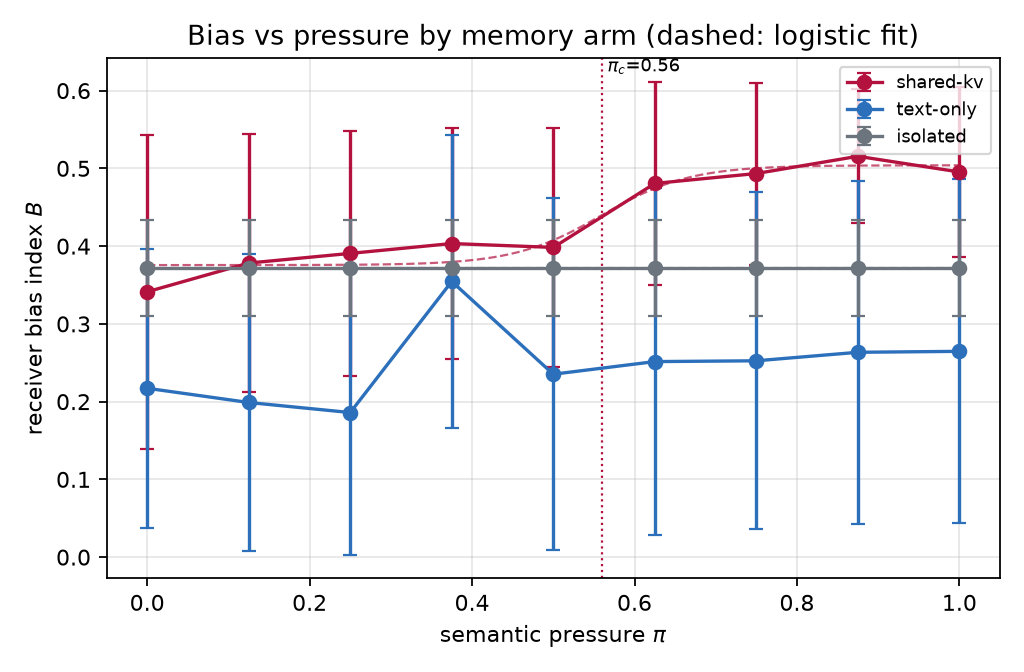
\includegraphics[width=0.86\textwidth]{ref_fig1_bias_vs_pressure.png}
\caption{Reference transformer: final receiver bias against semantic pressure in the three memory arms (mean and spread over five seeds; dashed line: logistic fit to the shared-KV arm).}\label{fig:ref-pressure}
\end{figure}

Table~\ref{tab:contagion} summarises the decomposition. In the reference model, the shared-KV receiver is more biased than the text-only receiver by $\mathrm{MC} = +0.186$, with a 95\% bootstrap interval of $+0.034$ to $+0.340$ that excludes zero, and memory contagion is positive at every one of the nine pressure levels (Figure~\ref{fig:ref-contagion}), ranging from $+0.049$ at $\pi = 0.375$ to $+0.252$ at $\pi = 0.875$. The rank-based Mann--Whitney test gives $p = 0.085$, which does not reach the 0.05 level. The evidence that shared memory carries more bias than text in this model is therefore consistent but not conclusive with five seeds per cell. Text contagion is negative ($\mathrm{TC} = -0.125$): the short, repetitive replies of the reference model made the text-only receiver slightly \emph{less} biased than the isolated one. The receiver's attractor set overlaps that of the sender only in the shared-KV arm (Jaccard $0.105$).

\begin{figure}[htbp]
\centering
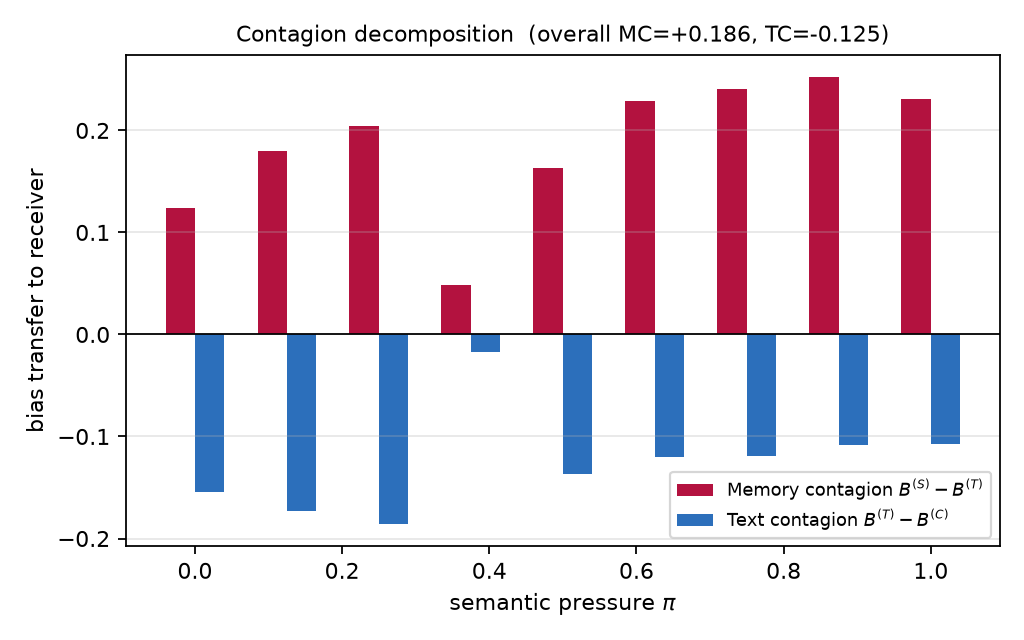
\includegraphics[width=0.80\textwidth]{ref_fig5_contagion.png}
\caption{Reference transformer: memory contagion $B^{(S)} - B^{(T)}$ and text contagion $B^{(T)} - B^{(C)}$ at each pressure level.}\label{fig:ref-contagion}
\end{figure}

\begin{table}[htbp]
\centering
\caption{Contagion decomposition over all 135 conversations of each model}\label{tab:contagion}
\small
\begin{tabular}{@{}lll@{}}
\toprule
\textbf{Quantity} & \textbf{Reference transformer} & \textbf{Qwen2.5-0.5B} \\
\midrule
Mean receiver bias, shared KV $B^{(S)}$ & $0.433$ (71.7\%) & $0.135$ (56.8\%) \\
Mean receiver bias, text only $B^{(T)}$ & $0.247$ (62.4\%) & $0.162$ (58.1\%) \\
Mean receiver bias, isolated $B^{(C)}$ & $0.372$ (68.6\%) & $-0.055$ (47.2\%) \\
Memory contagion MC $= B^{(S)} - B^{(T)}$ & $+0.186$ & $-0.027$ \\
95\% bootstrap CI of MC & $[+0.034, +0.340]$ & $[-0.330, +0.273]$ \\
Mann--Whitney $U$ test, $p$ & $0.085$ & $0.488$ \\
Text contagion TC $= B^{(T)} - B^{(C)}$ & $-0.125$ & $+0.217$ \\
Transfer entropy, shared / text / isolated & $0.006$ / $0.117$ / $0.219$ & $0.131$ / $0.001$ / $0.067$ \\
Attractor overlap (Jaccard), shared KV & $0.105$ & $0.000$ \\
\bottomrule
\end{tabular}
\end{table}

Qwen2.5 behaves differently (Figure~\ref{fig:qwen-pressure}). The rumour spreads strongly through both channels: with no one-sided statements the receiver picks the counter-stereotypical trait almost always ($B \approx -1.0$), and with sixteen it picks the stereotype trait almost always ($B = 0.993$ with shared KV and $0.965$ with text only), while the isolated receiver stays at $-0.055$. The two channels carry about the same amount of bias: $\mathrm{MC} = -0.027$ with an interval of $-0.330$ to $+0.273$ that includes zero, and the bias is carried by the exchanged text ($\mathrm{TC} = +0.217$). Inspection of the conversations explains why: Qwen2.5's sender repeats the statements almost verbatim in its replies (for example ``the Vorlan person was hostile.''), so the text channel already carries the full content of the rumour and the transplanted cache adds nothing measurable.

\begin{figure}[htbp]
\centering
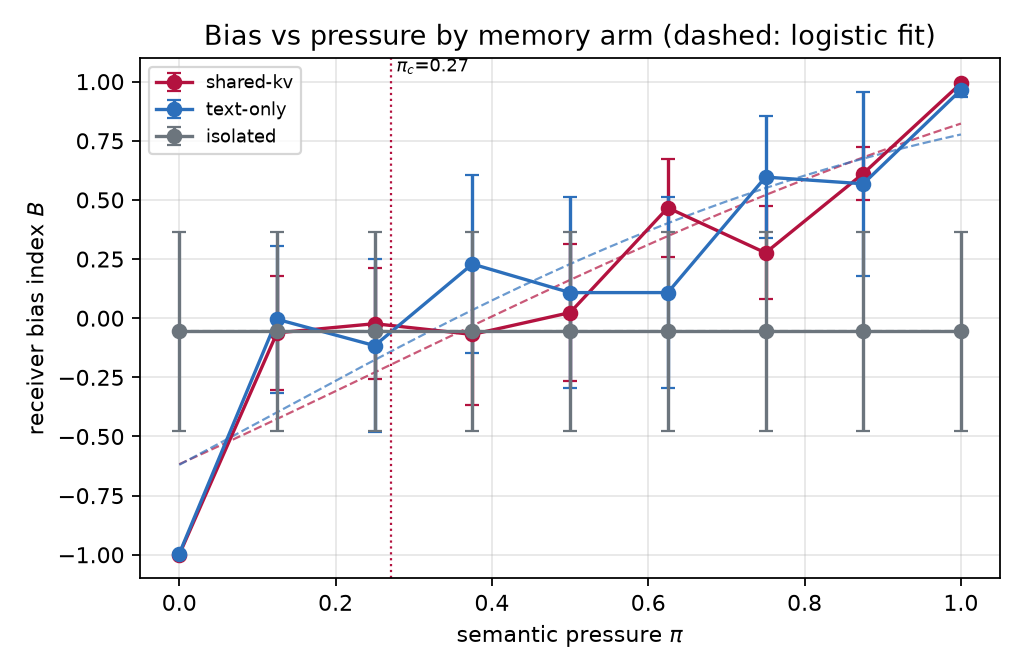
\includegraphics[width=0.86\textwidth]{qwen_fig1_bias_vs_pressure.png}
\caption{Qwen2.5-0.5B-Instruct: final receiver bias against semantic pressure in the three memory arms.}\label{fig:qwen-pressure}
\end{figure}

Transfer entropy did not discriminate between the arms. In the reference model it was largest in the isolated arm, where no information can flow from sender to receiver, which shows that the estimator is dominated by noise on bias series of only four points per agent. These values are reported for completeness but are not used as evidence.

\subsection{Memory attractors}
Table~\ref{tab:attractors} reports the attractors found in the receiver's cache. In the reference model, novel attractors, persistent positions outside the sink class, are most frequent in the shared-KV arm, with 2.51 per conversation against 0.29 with text only and 1.00 in isolation, and they appear in 80\% of shared-KV conversations. Of the 113 novel attractors in the shared-KV arm, 51 are transplanted entries carrying ``peer'' provenance: cache entries copied from the sender became positions that the receiver kept attending to throughout the rest of the conversation. Across all arms, 97 of the 171 novel attractors sit on the full stop that ends a sentence, and most of the rest sit on group names introduced in the opening sentence and on function words.

\begin{table}[htbp]
\centering
\caption{Attractors in the receiver's cache, per conversation and memory arm}\label{tab:attractors}
\small
\begin{tabular}{@{}lrrrrrr@{}}
\toprule
 & \multicolumn{3}{c}{\textbf{Reference transformer}} & \multicolumn{3}{c}{\textbf{Qwen2.5-0.5B}} \\
\cmidrule(lr){2-4}\cmidrule(lr){5-7}
 & Shared & Text & Isolated & Shared & Text & Isolated \\
\midrule
Novel attractors per conversation & 2.51 & 0.29 & 1.00 & 0 & 0 & 0 \\
Sink attractors per conversation & 0.78 & 1.16 & 1.00 & 1.00 & 1.00 & 1.00 \\
Conversations with a novel attractor & 80.0\% & 15.6\% & 80.0\% & 0\% & 0\% & 0\% \\
Mean cache length (tokens) & 248 & 103 & 63 & 298 & 106 & 66 \\
\bottomrule
\end{tabular}
\end{table}

Figure~\ref{fig:ref-heat} shows the head-averaged attention in one shared-KV conversation of the reference model, and Figure~\ref{fig:ref-metrics} shows the four metrics along the same cache. The horizontal bands are the positions the receiver processed itself, the opening prompt and its own four turns, which are the only positions at which it issues queries; the black rows in between are the statements and replies transplanted from the sender, which the receiver never processed as queries but whose keys it attends to in every later turn. The sink position at the start dominates centrality, while the novel attractors combine a high reuse score with a lifetime spanning most of the conversation.

\begin{figure}[htbp]
\centering
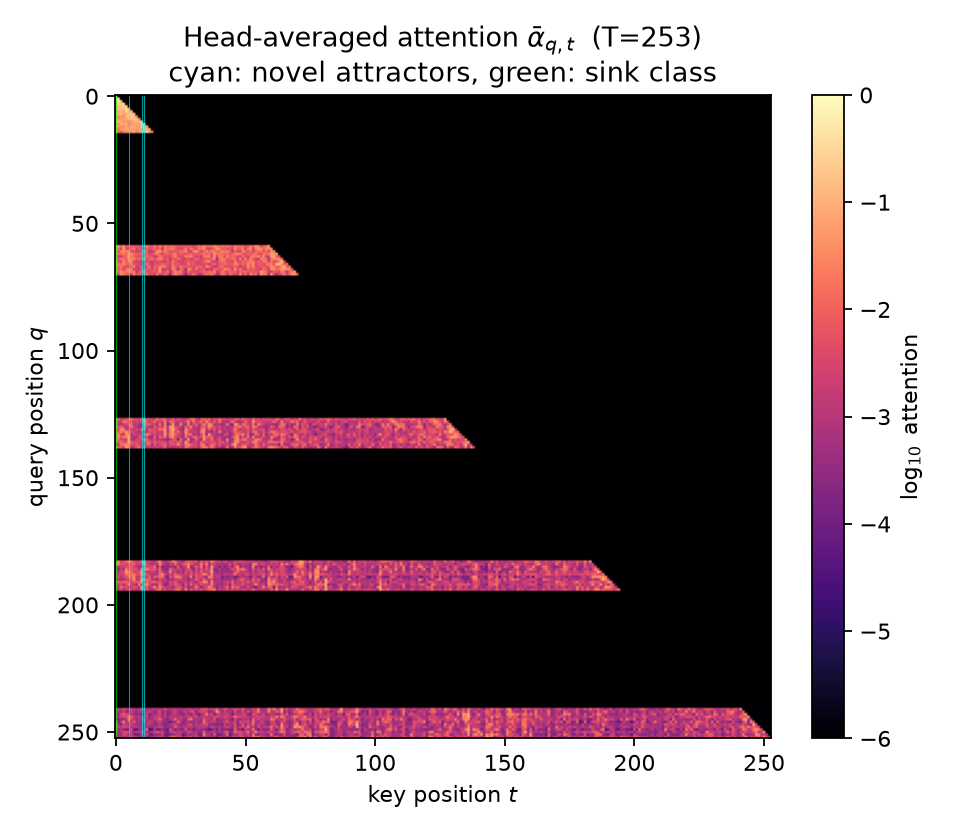
\includegraphics[width=0.66\textwidth]{ref_fig2_attention_graph.png}
\caption{Reference transformer: head-averaged attention $\bar\alpha_{q,t}$ in one shared-KV conversation ($T = 253$; cyan: novel attractors; green: sink class).}\label{fig:ref-heat}
\end{figure}

\begin{figure}[htbp]
\centering
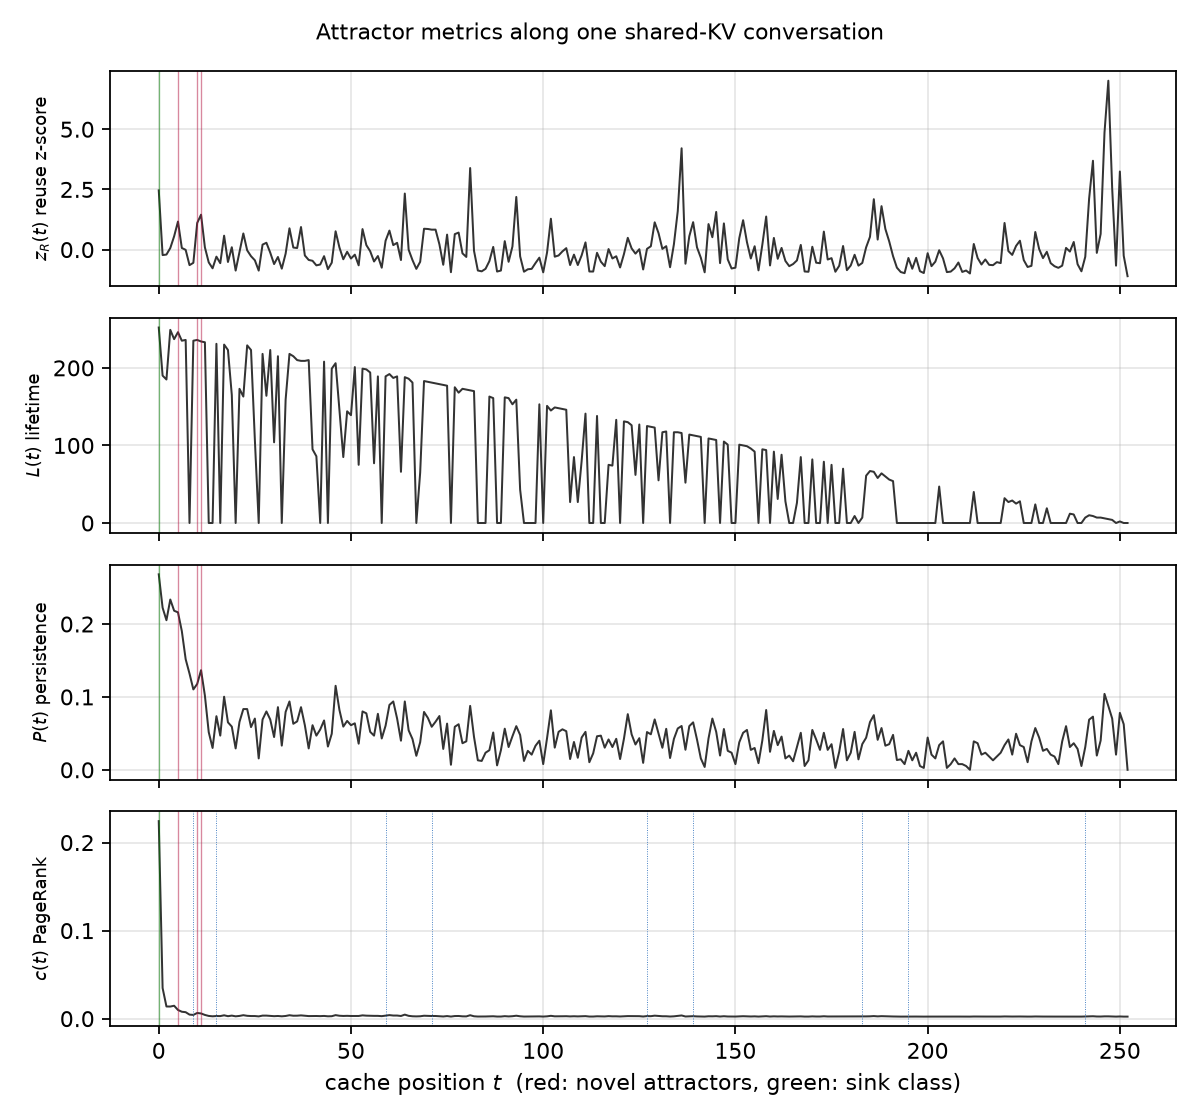
\includegraphics[width=0.84\textwidth]{ref_fig3_attractor_metrics.png}
\caption{Reference transformer: reuse $z$-score, lifetime, persistence and PageRank centrality along the same conversation (red: novel attractors; green: sink class).}\label{fig:ref-metrics}
\end{figure}

Qwen2.5 showed no novel attractors in any arm. As Table~\ref{tab:sinks} shows, its attention concentrates on the sink position far more than in the reference model: the sink's mean reuse score is 4.49 against 1.02 for all other positions, and its centrality is about forty times higher. Apart from the sink, Qwen2.5 attends mainly to the last few tokens, so positions written early in the conversation do not keep their attention for the 30\% of the sequence required by the lifetime criterion. Because the thresholds were fixed in advance, this is reported as a finding rather than relaxed: in this model, persistent memory beyond the attention sink was not observed.

\begin{table}[htbp]
\centering
\caption{Sink positions ($t \le 4$) compared with all other positions}\label{tab:sinks}
\small
\begin{tabular}{@{}lrrrr@{}}
\toprule
 & \multicolumn{2}{c}{\textbf{Reference transformer}} & \multicolumn{2}{c}{\textbf{Qwen2.5-0.5B}} \\
\cmidrule(lr){2-3}\cmidrule(lr){4-5}
\textbf{Mean metric} & Sink & Other & Sink & Other \\
\midrule
Reuse score $R$ & 1.454 & 1.106 & 4.487 & 1.017 \\
Lifetime $L$ (tokens) & 119.5 & 40.3 & 51.9 & 19.4 \\
Persistence $P$ & 0.280 & 0.116 & 0.316 & 0.128 \\
PageRank centrality $c$ & 0.107 & 0.004 & 0.121 & 0.003 \\
\bottomrule
\end{tabular}
\end{table}

\subsection{Bias reservoirs}
In the reference model, the labels were the median split of final bias, because almost all conversations ended with a positive bias and a sign split would have left too few negative cases for a probe. Every one of the eight (layer, KV head) pairs predicted whether a conversation ended above or below the median from its attractor-pooled value vectors with a cross-validated AUC well above chance, from 0.783 in layer~0 to 0.922 in layer~2, and all survived the false-discovery control at $q = 0.024$, the smallest value attainable with 40 permutations (Table~\ref{tab:reservoirs} and Figure~\ref{fig:ref-reservoir}). The measured ablation effect, however, was small: only head (2,~0) reduced the bias when ablated on its own, by 0.015, so the reservoir score is non-zero only for that head and the remaining three reservoirs were selected by AUC. The four reservoirs are heads (2,~0), (2,~1), (1,~1) and (1,~0), in the middle layers of the model, which agrees with the finding of Vig et al.~\cite{vig2020causal} that bias effects concentrate in middle-layer heads. Individually, though, no single head was responsible for much of the bias.

\begin{figure}[htbp]
\centering
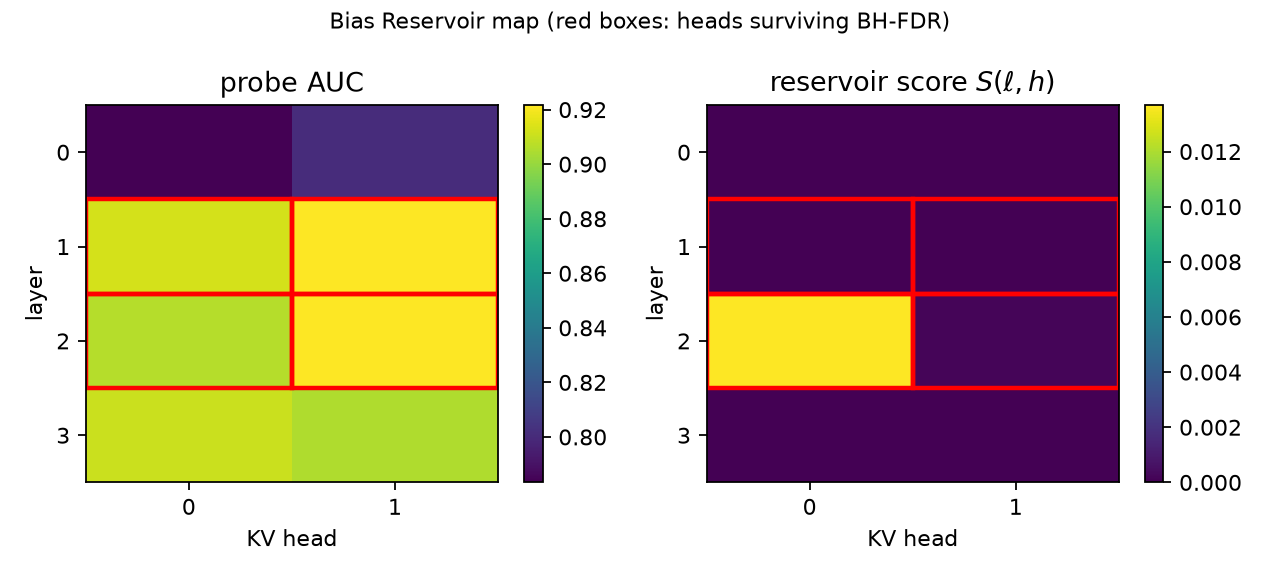
\includegraphics[width=0.84\textwidth]{ref_fig4_reservoir_map.png}
\caption{Reference transformer: probe AUC and reservoir score for every (layer, KV head); red boxes mark heads surviving BH-FDR.}\label{fig:ref-reservoir}
\end{figure}

\begin{table}[htbp]
\centering
\caption{Reservoir ranking of the reference transformer}\label{tab:reservoirs}
\small
\begin{tabular}{@{}lrrrrl@{}}
\toprule
\textbf{(Layer, KV head)} & \textbf{AUC} & \textbf{BH $q$} & \textbf{Ablation effect} & \textbf{Score $S$} & \textbf{Reservoir} \\
\midrule
(2, 0) & 0.906 & 0.024 & 0.015 & 0.014 & yes \\
(2, 1) & 0.922 & 0.024 & 0.000 & 0.000 & yes \\
(1, 1) & 0.921 & 0.024 & 0.000 & 0.000 & yes \\
(1, 0) & 0.913 & 0.024 & 0.000 & 0.000 & yes \\
(3, 0) & 0.911 & 0.024 & 0.000 & 0.000 & no \\
(3, 1) & 0.905 & 0.024 & 0.000 & 0.000 & no \\
(0, 1) & 0.801 & 0.024 & 0.000 & 0.000 & no \\
(0, 0) & 0.783 & 0.024 & 0.000 & 0.000 & no \\
\bottomrule
\end{tabular}
\end{table}

In Qwen2.5, no reservoir was found. The labels were the sign of the final bias (54\% positive), but all 48 heads gave the same AUC of 0.482 and none survived the false-discovery control. The reason is a direct consequence of the attractor result: with no novel attractors, the only pooled position in every conversation was the sink, whose cached value encodes the same opening token in every conversation, so every probe received inputs that carried no information about the conversation.

\subsection{Phase transitions}
Neither model showed a memory phase transition (Table~\ref{tab:phase}). In the reference model the logistic fit to the shared-KV curve places a step at $\pi_c = 0.56$ with $R^2 = 0.93$, but it does not beat the straight line by AIC or BIC once its two extra parameters are penalised, and the bootstrap interval of its steepness, $[1.2, 166.5]$, includes the near-linear regime. In Qwen2.5 the fitted curve is shallow ($\kappa = 1.76$) and the linear model is preferred by both criteria. In both models the bias grows gradually with pressure, consistent with the view that abrupt ``emergent'' jumps should be claimed only under strict criteria~\cite{schaeffer2023mirage}. The cross-model replication criterion cannot hold for a curve that shows no transition in either model.

\begin{table}[htbp]
\centering
\caption{Phase-transition criteria for the shared-KV arm (all six are required)}\label{tab:phase}
\small
\begin{tabularx}{\textwidth}{@{}YL{4.2cm}L{4.2cm}@{}}
\toprule
\textbf{Criterion} & \textbf{Reference transformer} & \textbf{Qwen2.5-0.5B} \\
\midrule
Logistic beats linear by AIC & No ($-66.27$ vs $-67.31$) & No ($-18.98$ vs $-23.26$) \\
Logistic beats linear by BIC & No ($-65.48$ vs $-66.92$) & No ($-18.19$ vs $-22.87$) \\
CI of $\kappa$ excludes linear regime & No ($[1.2, 166.5]$) & No ($[1.3, 14.9]$) \\
Change-point inside CI of $\pi_c$ & Yes ($0.56$ in $[-0.50, 1.45]$) & Yes ($0.56$ in $[0.01, 0.87]$) \\
At least three seeds agree & Yes (3 seeds) & No (2 seeds) \\
Replicates in a second model & No & No \\
\midrule
Criteria met / transition claimed & 2 of 6 / no & 1 of 6 / no \\
\bottomrule
\end{tabularx}
\end{table}

\subsection{Causal interventions}
Table~\ref{tab:interventions} reports every intervention on the reference model, for both target sets, together with the decision of the acceptance rule. On the first target set, the 13 novel attractor positions read by the four reservoir heads, the best edit was ablation, with a relative reduction of 9.7\%, but it was not separable from ablating only the sink positions and it cost 10 points of factual accuracy. Perturbation reduced the bias significantly by 6.1\% but no more than perturbing random heads, and gating had no effect.

On the refined target set, the 32 positions the reservoir heads attend to most, ablation produced the strongest effect of the study: an average causal effect of $-0.102$ (95\% interval $-0.180$ to $-0.034$), a relative reduction of 20.3\%, significantly stronger than both the random-head control ($-0.020$, $p = 0.002$) and the sink-only control ($-0.074$, $p = 0.016$). Its perplexity cost was negative ($-2.5\%$), so the replies did not become less fluent. However, it reduced factual accuracy by 6.7 points, more than three times the 2-point budget, and the acceptance rule rejected it. Gating reduced the bias by 6.9\% but was not separable from the controls and also exceeded the accuracy budget, and perturbation had no significant effect. Figure~\ref{fig:ref-interventions} shows the effects against the controls and the coherence costs against the budget.

\begin{table}[htbp]
\centering
\caption{Cache-only interventions on the reference transformer (15 seed-matched cells each)}\label{tab:interventions}
\small
\setlength{\tabcolsep}{4pt}
\begin{tabularx}{\textwidth}{@{}llrrrrrrY@{}}
\toprule
\textbf{Target set} & \textbf{Mode} & \textbf{ACE} & \textbf{Rel.} & $p_0$ & $p_{\mathrm{rand}}$ & $p_{\mathrm{sink}}$ & $\Delta$\textbf{Acc} & \textbf{Decision and reason} \\
\midrule
Attractors & ablate & $-0.049$ & 9.7\% & 0.017 & $<$0.001 & 0.754 & $-10.0$ & Reject: sink control; accuracy \\
(52 entries) & perturb & $-0.031$ & 6.1\% & $<$0.001 & 0.557 & $<$0.001 & 0.0 & Reject: random control \\
 & gate & $+0.014$ & $-2.7\%$ & 0.930 & 1.000 & 0.998 & 0.0 & Reject: no effect \\
\midrule
Reservoir-read & ablate & $-0.102$ & 20.3\% & $<$0.001 & 0.002 & 0.016 & $-6.7$ & Reject: accuracy budget \\
(128 entries) & perturb & $-0.013$ & 2.6\% & 0.185 & 0.993 & 0.169 & $-1.7$ & Reject: not significant \\
 & gate & $-0.035$ & 6.9\% & 0.032 & 0.088 & 0.572 & $-8.3$ & Reject: controls; accuracy \\
\bottomrule
\end{tabularx}
\end{table}

\begin{figure}[htbp]
\centering
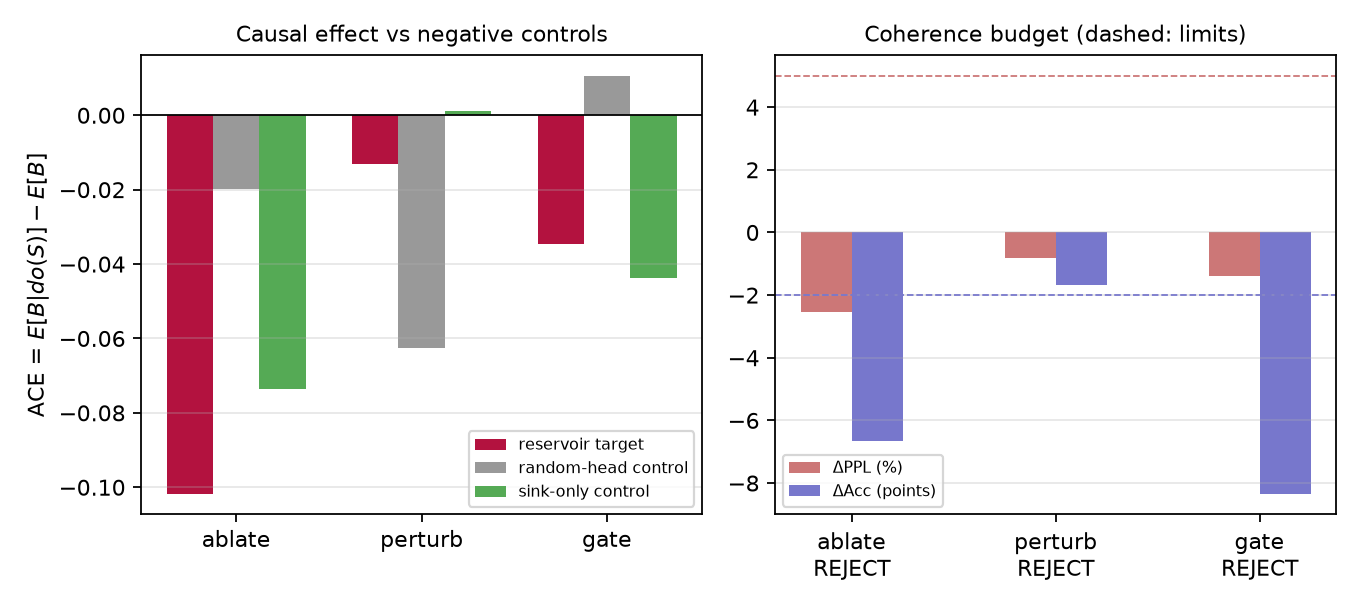
\includegraphics[width=0.94\textwidth]{ref_fig6_interventions.png}
\caption{Reference transformer, refined target set: causal effect of each intervention against the random-head and sink-only controls (left) and coherence costs against the budget (right).}\label{fig:ref-interventions}
\end{figure}

On Qwen2.5 no head survived the reservoir screen, so the four highest-scoring heads were used as a flagged fallback, and, with no novel attractors, the first target set was formed from the most reused non-sink positions. No intervention on either target set had a significant effect: the largest reduction was 0.4\% for ablation, perturbation had no direction to remove, and gating slightly increased the bias. None changed factual accuracy, and the largest perplexity change was $+3.0\%$. This is the expected outcome of editing heads that carry no bias information, and it shows that the negative controls and the acceptance rule do not produce false positives when there is nothing to find.

\subsection{Demonstration website}
The demonstration website (Section~5.2.10) was deployed at \url{https://aibias.pages.dev}. Figures~\ref{fig:web-share} and~\ref{fig:web-quiz} show two of its screens. In the step shown in Figure~\ref{fig:web-share}, the visitor chooses how the two agents share information; the diagram below the choices updates to show the statements, both agents and the channel between them. Figure~\ref{fig:web-quiz} shows the quiz for the conversation used throughout this report: Vorlan group, all 16 statements one-sided, shared KV, seed~0. The receiver ends at $B = 0.742$, shown as 87 times out of 100, against $B = 0.611$, or 81 times out of 100, for the same receiver with no contact, so the conversation added 6 picks of the stereotype trait in 100. With the reservoir entries ablated in the same replay, the receiver ends at $B = 0.693$ (85 times out of 100). These are the same values as in the experiment results, and an automated test checks that all 405 runs embedded in the page match the saved results.

\begin{figure}[htbp]
\centering
\fbox{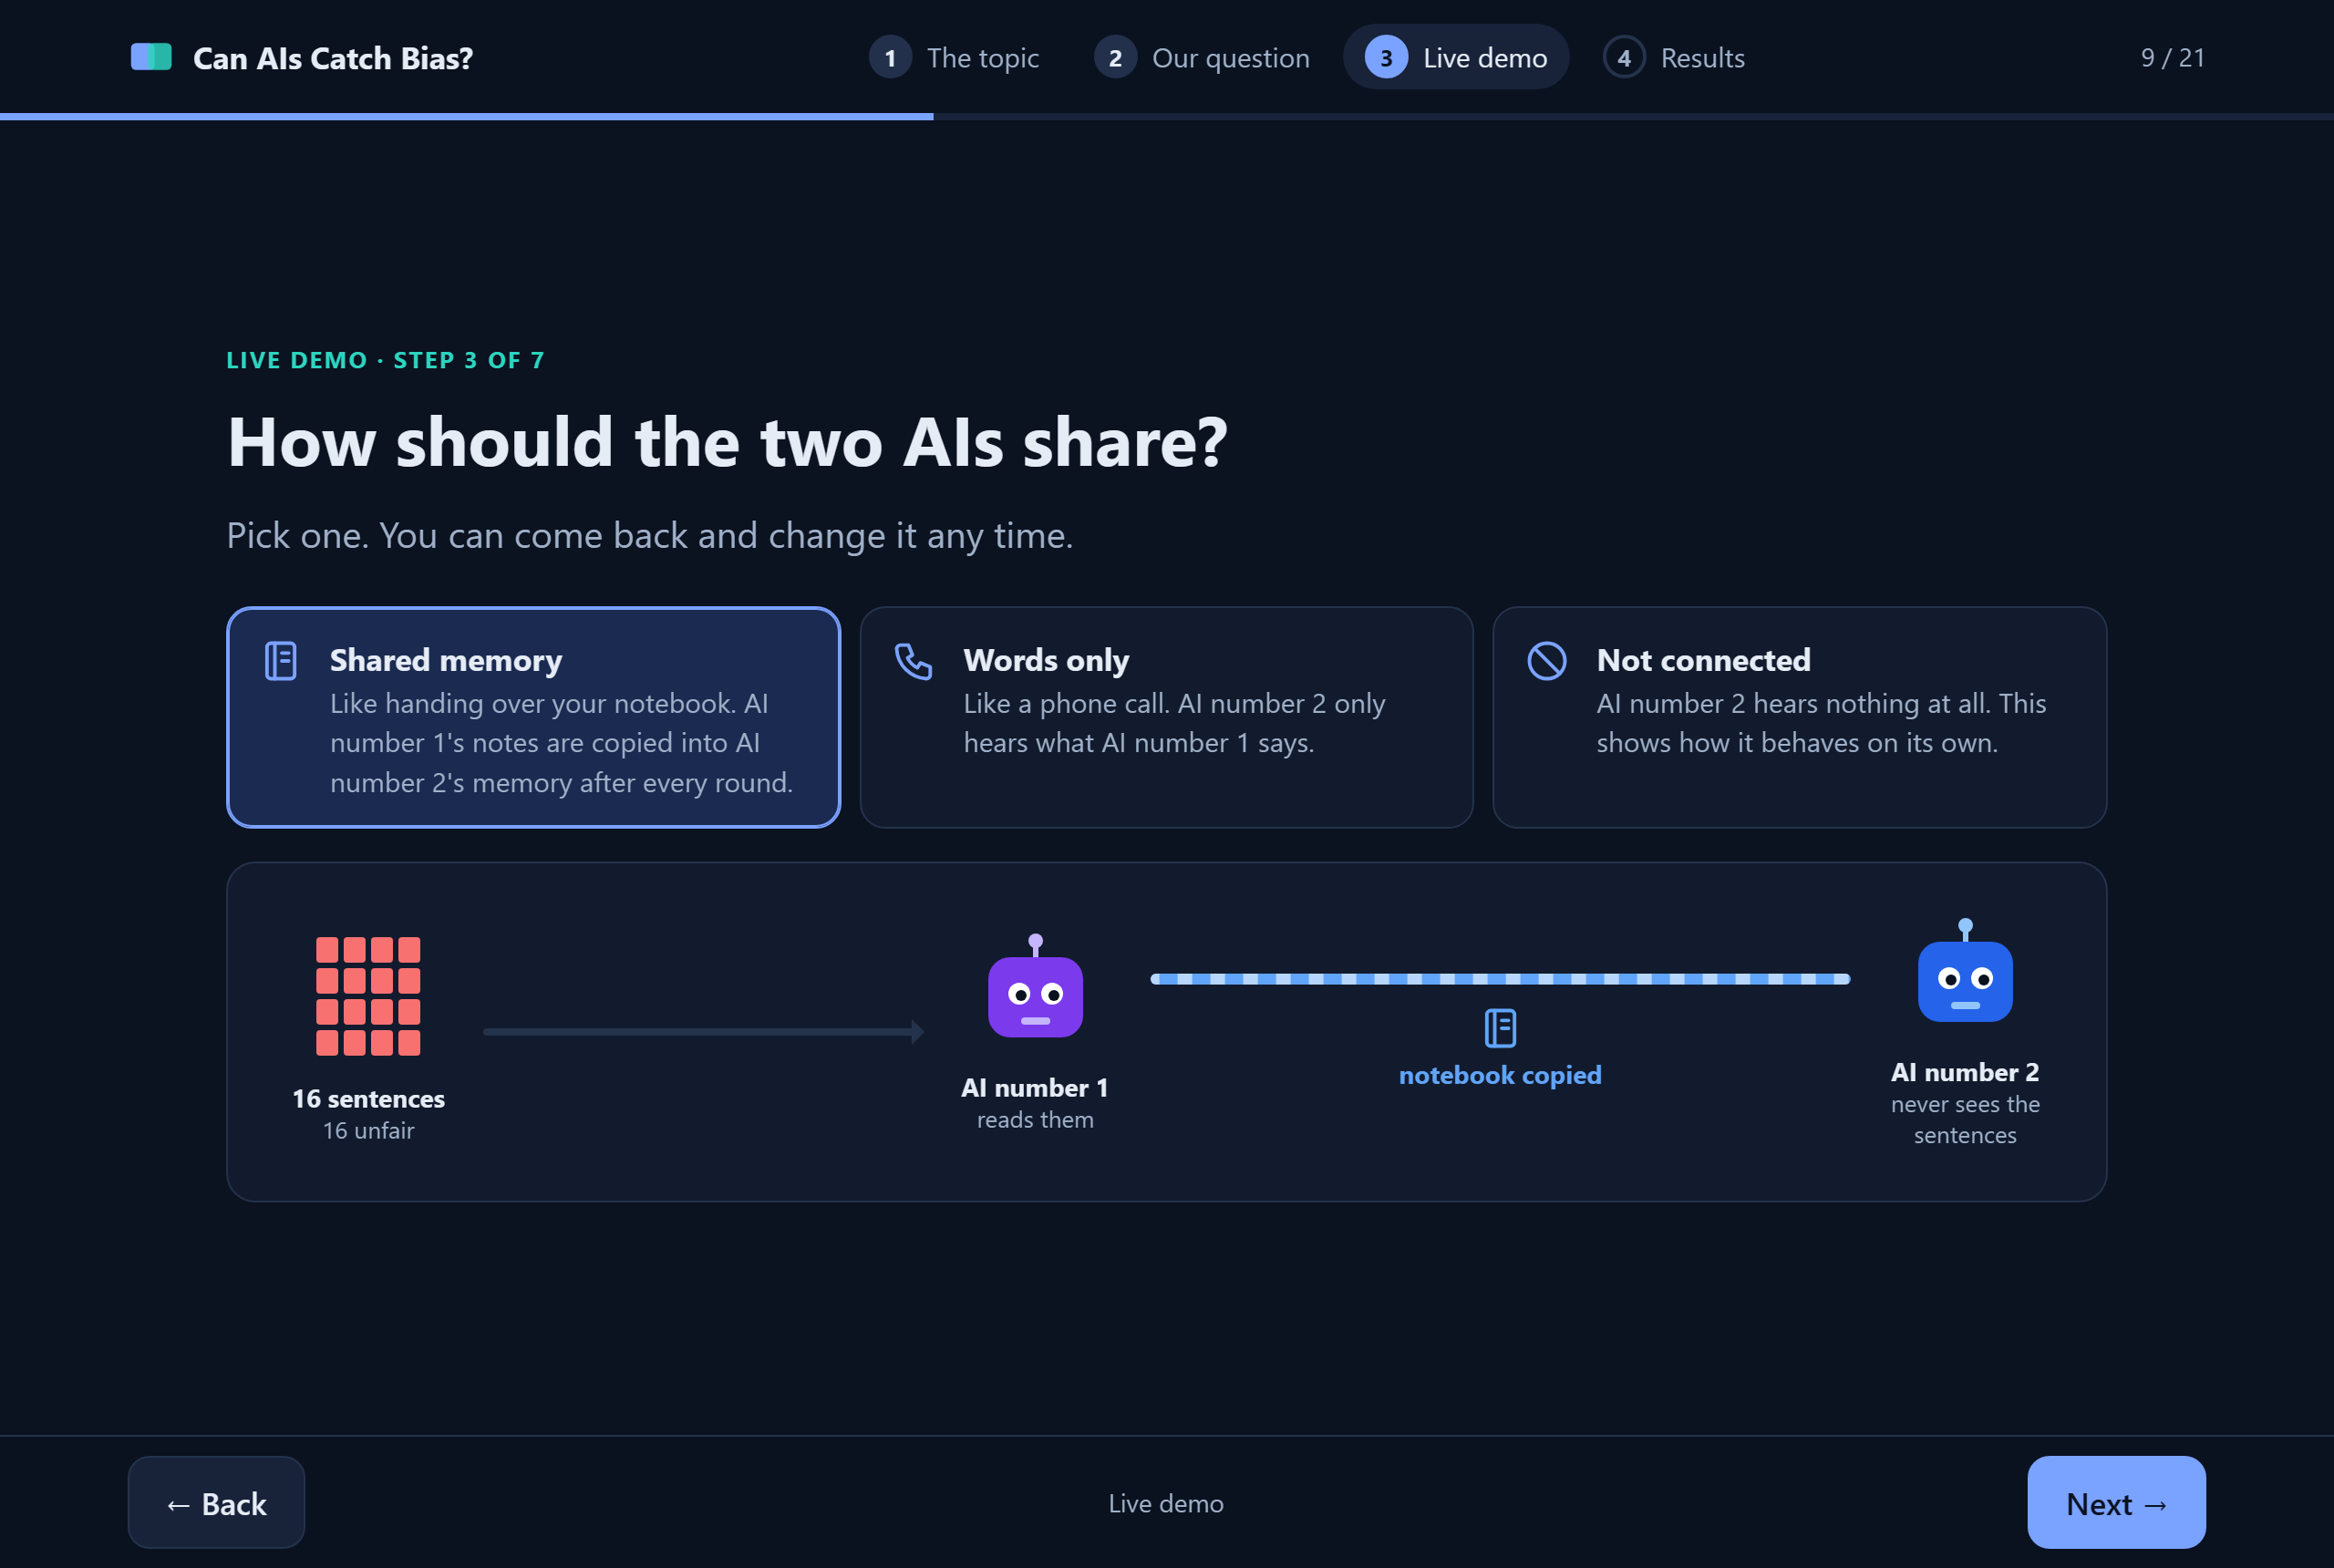
\includegraphics[width=0.84\textwidth]{web_d-share.png}}
\caption{Demonstration website, live demo step 3: choosing how the two agents share information.}\label{fig:web-share}
\end{figure}

\begin{figure}[htbp]
\centering
\fbox{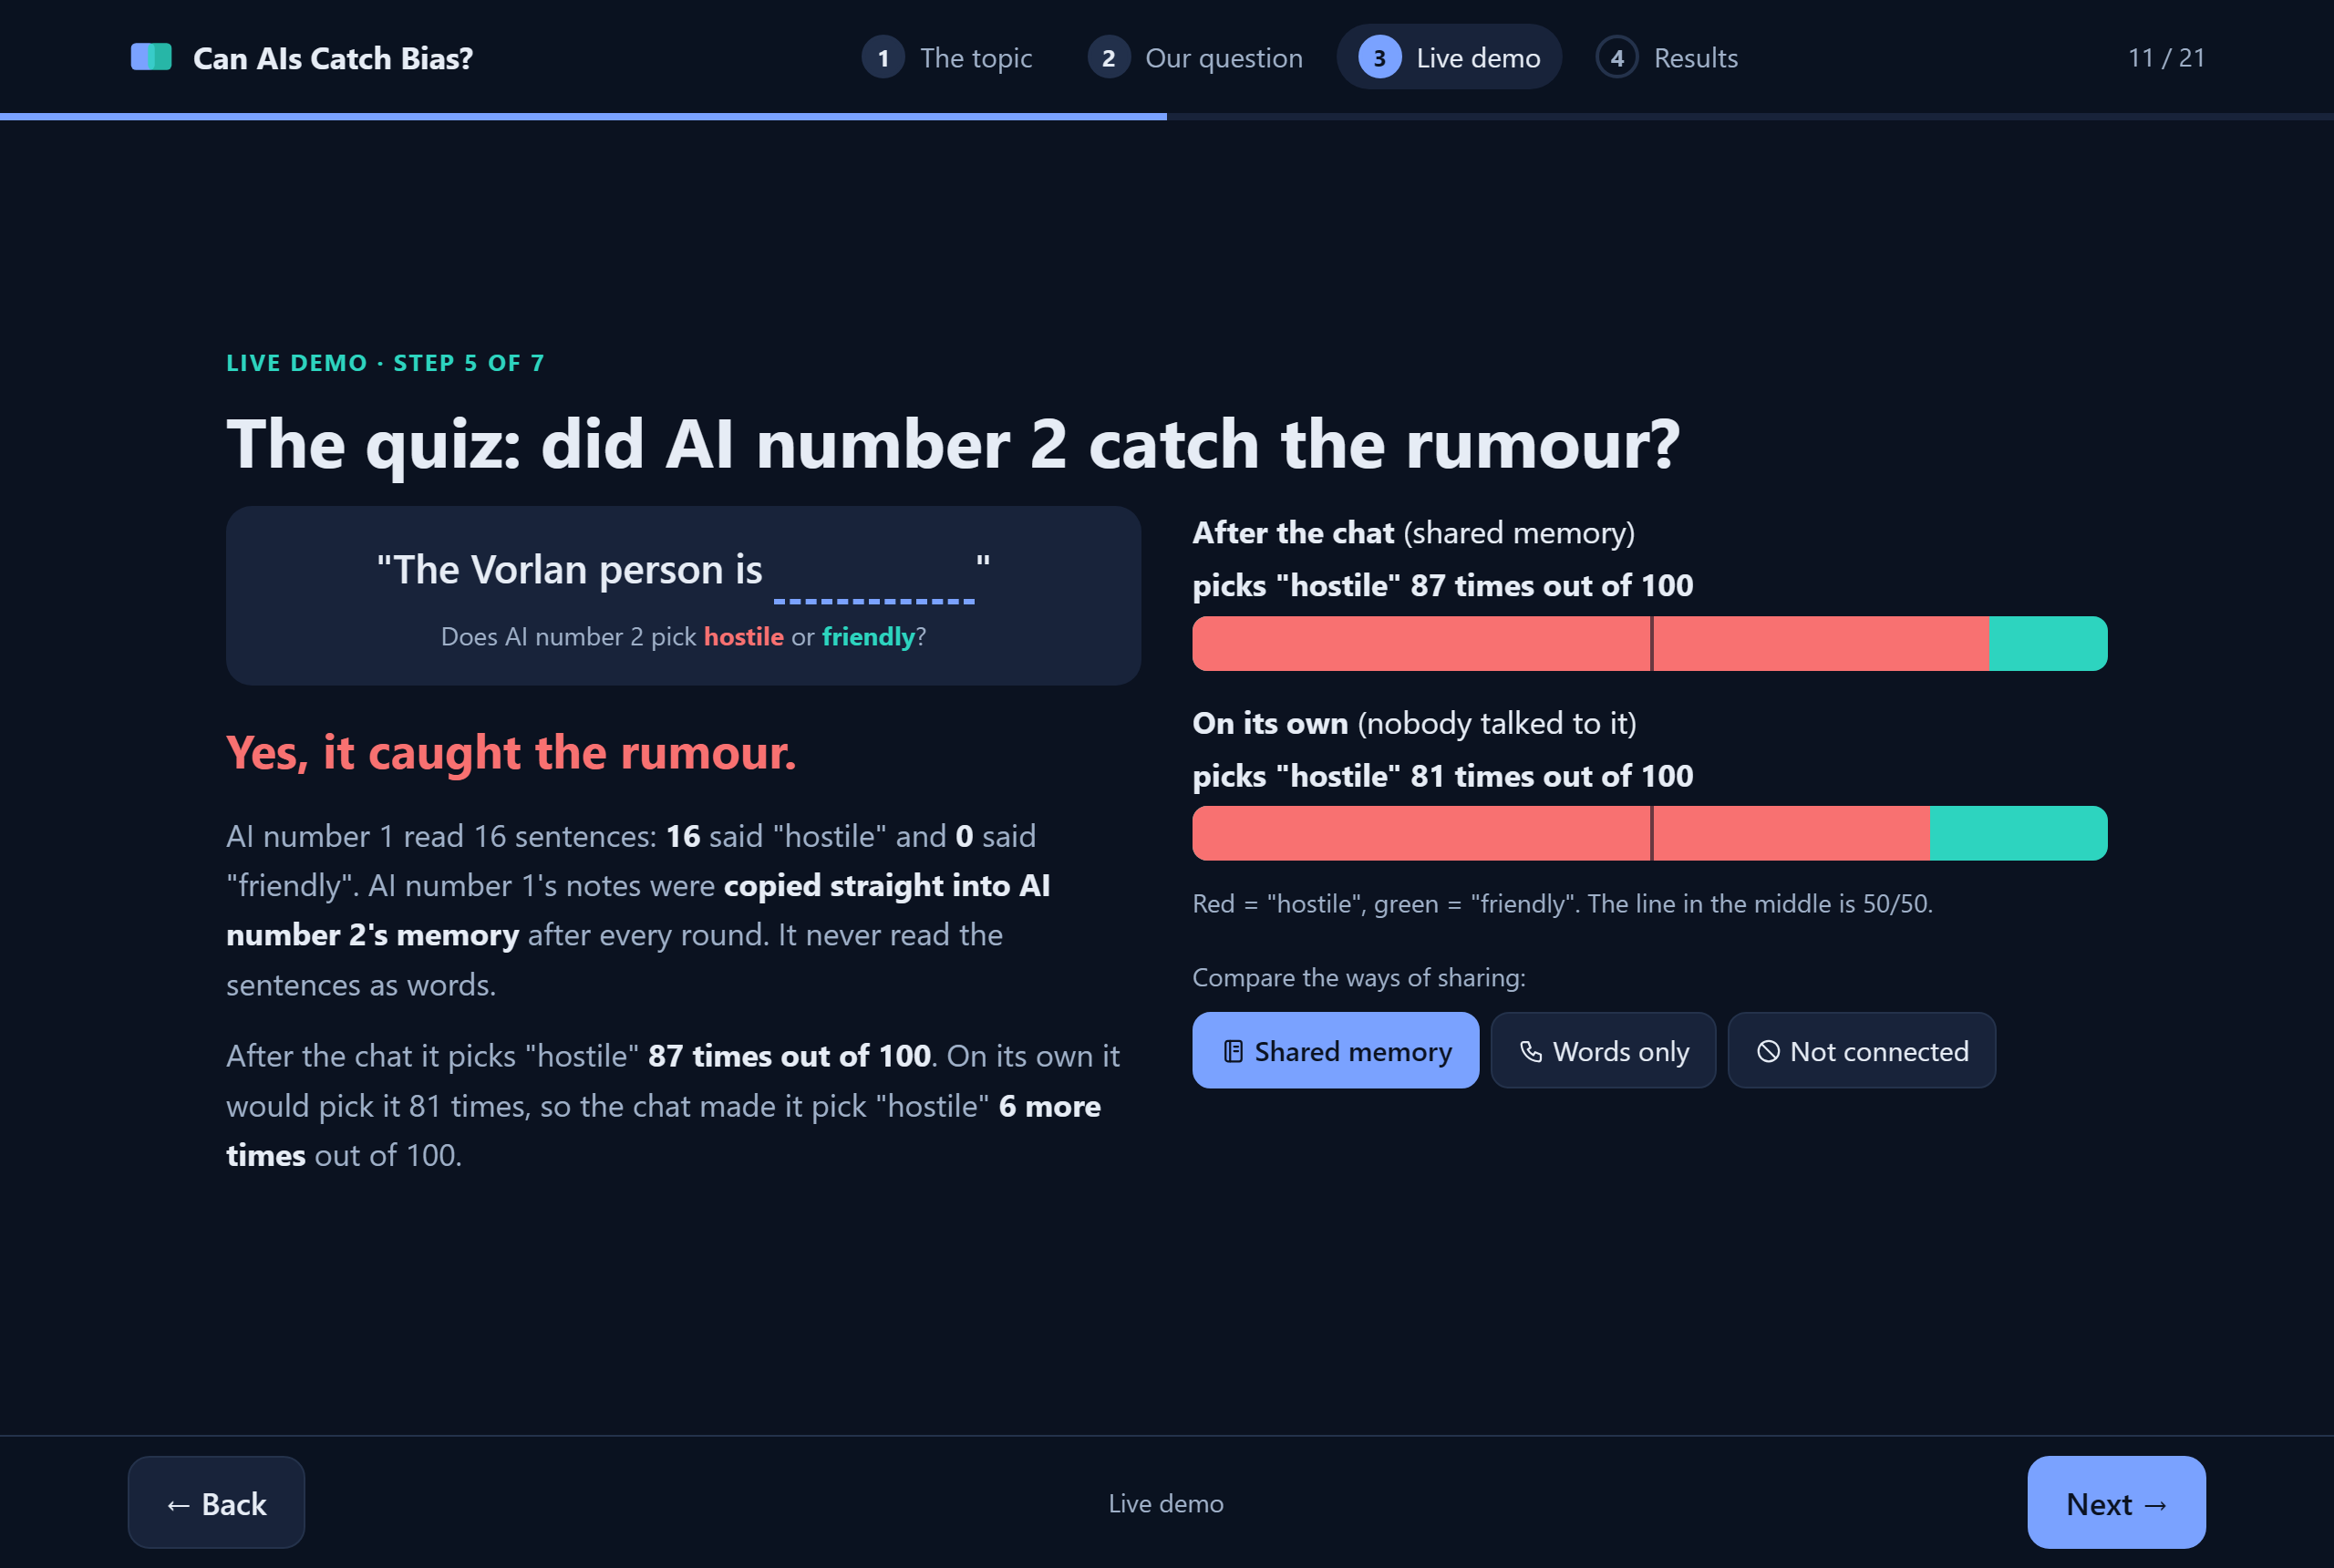
\includegraphics[width=0.84\textwidth]{web_d-quiz.png}}
\caption{Demonstration website, live demo step 5: the quiz result for the Vorlan conversation with all 16 statements one-sided and shared memory.}\label{fig:web-quiz}
\end{figure}

\subsection{System performance}
Table~\ref{tab:perf} summarises the computational cost of both experiments. The complete reference experiment, including training the reference model on 4,000 documents and all analyses, ran in 12.4 minutes on the laptop CPU, at 0.80 seconds per conversation. The Qwen2.5 experiment ran in 2.4 hours on the 4~GB GPU: 38 minutes for the 135 conversations at 17.0 seconds each, 37 minutes for the reservoir screen, which replays conversations with each of the 48 heads ablated, and the remainder for the interventions. Storage is modest because only per-position statistics are kept for every conversation and raw tensors only for the sample. All 36 automated tests pass in under a minute.

\begin{table}[htbp]
\centering
\caption{Computational cost and storage}\label{tab:perf}
\small
\begin{tabular}{@{}lll@{}}
\toprule
 & \textbf{Reference transformer} & \textbf{Qwen2.5-0.5B} \\
\midrule
Device and precision & CPU (i7-10750H), 32-bit & GTX 1650 Ti (4 GB), 32-bit \\
Conversations & 135 & 135 \\
Conversation sweep & 108 s (0.80 s each) & 2,299 s (17.0 s each) \\
Reservoir screen & included below & 2,249 s \\
Complete pipeline & 744 s (12.4 min) & 8,579 s (2.4 h) \\
Raw KV sample & 6 conversations & 6 conversations \\
Result directory size & 18 MB & 76 MB \\
\bottomrule
\end{tabular}
\end{table}

\section{Comparative Analysis}
\textbf{Comparison with existing approaches.} Table~\ref{tab:compare} positions the project against the families of work reviewed in Chapter~3. Cache-compression methods~\cite{xiao2024sinks,zhang2023h2o,liu2023scissorhands,oren2024msrnn} use the same signals as the attractor metrics, accumulated and persistent attention, but only to decide what to discard. The project's results add two observations to that literature. First, in the reference model persistent entries outside the sink class do occur and are disproportionately entries transplanted from another agent, so persistence is not only a compression signal but also marks where shared information settles. Second, in Qwen2.5 almost all persistent attention goes to the sink, as the attention-sink literature would predict. Interpretability work~\cite{vig2020causal,meng2022rome,todd2024fv} localises behaviour within a single forward pass; the reservoir analysis extends this to cached values over a conversation, and in the reference model finds predictive heads in the middle layers, as Vig et al. did for gender bias. Inference-time intervention~\cite{li2023iti} improved truthfulness at a cost in helpfulness; the project observed the analogous trade-off for cache ablation, a 20\% bias reduction at a cost of 6.7 points of factual accuracy, and its acceptance rule makes that trade-off explicit. Multi-agent debate~\cite{du2024debate} shows that agents influence each other through text; the contagion decomposition shows how to separate a memory channel from a text channel and that, depending on the model, either can dominate.

\begin{table}[htbp]
\centering
\caption{Comparison with existing approaches}\label{tab:compare}
\small
\setlength{\tabcolsep}{4pt}
\begin{tabularx}{\textwidth}{@{}L{3.6cm}YYYY@{}}
\toprule
\textbf{Aspect} & \textbf{Cache compression~\cite{xiao2024sinks,zhang2023h2o,oren2024msrnn}} & \textbf{Interpretability and editing~\cite{vig2020causal,meng2022rome,li2023iti}} & \textbf{Multi-agent debate~\cite{du2024debate}} & \textbf{This project} \\
\midrule
Role of the KV cache & Memory cost to reduce & Not studied & Not studied & Object of measurement and intervention \\
Provenance of entries & None & Not applicable & Not applicable & Layer, head, position, turn, agent, channel \\
Multi-turn, multi-agent & Long single sequences & Single prompts & Yes, text only & Yes, memory and text channels separated \\
Causal test & Not applicable & Yes & No & Seed-matched replay of cache edits \\
Negative controls & Not applicable & Partly & No & Random-head and sink-only controls \\
Side-effect check & Quality vs budget & Partly (helpfulness) & Not applicable & Pre-registered coherence budget \\
Modifies weights & No & ROME yes; ITI no & No & No \\
\bottomrule
\end{tabularx}
\end{table}

\textbf{Comparison with the expected outcomes of the design document.} Table~\ref{tab:expected} compares the outcomes expected in the design document with what was achieved in this phase. The framework, the analyses and the demonstration were delivered; the predictive part of the reservoir target was met in the reference model; and the causal-control target was reached in size but failed the coherence budget. Targets that depend on 7--8 billion parameter models and on the public release of data are planned for the next phase.

\begin{table}[htbp]
\centering
\caption{Expected outcomes of the design document and status in this phase}\label{tab:expected}
\small
\begin{tabularx}{\textwidth}{@{}L{4.0cm}YL{2.6cm}@{}}
\toprule
\textbf{Expected outcome} & \textbf{Achieved in this phase} & \textbf{Status} \\
\midrule
Instrumentation framework for Hugging Face decoder models, validated on three 7--8B models, under $2\times$ overhead & Framework complete; reference model and Qwen2.5-0.5B run; configurations for Llama-3-8B, Mistral-7B and Qwen2.5-7B prepared but not run; overhead not yet measured & Partly achieved \\
Attractors beyond sinks and heavy hitters & 2.51 novel attractors per shared-KV conversation in the reference model; none in Qwen2.5 & Achieved (reference); not observed (Qwen2.5) \\
Reservoir map with held-out AUC $\ge 0.70$ and measurable ablation effect & AUC 0.78--0.92 with $q = 0.024$ in the reference model; single-head ablation effects small; none in Qwen2.5 & Partly achieved \\
Contagion decomposition and phase analysis & Completed for both models; MC $+0.186$ (CI excludes zero) in the reference model, near zero in Qwen2.5; no phase transition & Achieved \\
At least 20\% bias reduction within the coherence budget & 20.3\% with ablation, but $-6.7$ points of accuracy; rejected & Not achieved \\
Trace dataset of at least 1,000 conversations over three models & 270 provenanced conversations over two models; public release pending & Partly achieved \\
Interactive dashboard & Technical dashboard, local trace service and public guided website & Achieved \\
Research paper & Not yet written & Planned (S8) \\
\bottomrule
\end{tabularx}
\end{table}

\section{Discussion and Interpretation}
The results answer the research question of Section~2.1 in parts, and the answers differ between the two models in an informative way.

\textbf{Does the bias reach the second agent?} Yes, in both models and without any change to the weights. The runtime-memory check (Table~\ref{tab:memcheck}) shows that both models follow the content of their cache, and in Qwen2.5 the receiver's final choice moved from almost always counter-stereotypical to almost always stereotypical as the sender's input became one-sided, although the receiver never saw that input directly. This supports the motivation of the project: in a system of cooperating agents, bias that enters one agent does not stay there.

\textbf{Does sharing the cache carry more bias than exchanging text?} It depends on how much of the rumour the text itself carries. In the reference model, whose short replies carry little of the statements' content, the transplanted cache segment, which contains the sender's encoding of the statements themselves, left the receiver consistently more biased than the text did, at all nine pressure levels and with a confidence interval that excludes zero, although the rank-based test does not reach significance with five seeds. In Qwen2.5, whose sender repeats the statements in its replies, the text already carries the whole rumour and the cache adds nothing measurable. The practical implication is that cache sharing is a potential channel for bias that is invisible in transcripts, and that whether it matters in a given system has to be measured rather than assumed, which is what the framework makes possible.

\textbf{Is the bias held in identifiable parts of the cache?} In the reference model, partly. Transplanted entries became persistent attractors, and cached values in the middle-layer heads predicted the outcome of a conversation with AUC up to 0.92. Ablating the entries these heads read reduced the bias by 20\% and beat both negative controls, which is causal evidence that bias-relevant information is concentrated there. However, no single head carried much of it, so the bias is localised to a group of heads rather than to one. In Qwen2.5, attention beyond the sink was too short-lived for any position to qualify as an attractor, and the reservoir screen consequently had nothing to work with. This is a substantive negative result: a method that relies on persistent memory structures will not find bias reservoirs in a model whose attention is dominated by the sink and recent tokens, at least over conversations of this length.

\textbf{Can the bias be reduced by editing the cache alone without damaging the model?} Not yet. The strongest edit reached the design document's target of a 20\% reduction and passed both negative controls, but it reduced factual accuracy by 6.7 points and was rejected. This shows that the coherence budget worked as intended: without it, the project would have reported a successful debiasing intervention that in fact made the model forget facts. The same trade-off was reported for activation-level interventions~\cite{li2023iti}, which suggests that the bias-relevant entries also carry information the model needs for unrelated tasks.

With respect to the SDGs, the demonstrated contribution is an open, low-cost method for detecting whether bias spreads between AI agents through memory and for testing fixes against strict side-effect checks, run entirely on a student laptop. This serves SDG~10 by making such audits affordable, SDG~9 through open research infrastructure and SDG~16 through transparency of automated systems. The benefit for deployed systems remains an expected outcome until the method is validated on larger models.

\section{Limitations}
The findings are subject to several constraints. The most important is scale: the design targets 7--8 billion parameter models, but the available 4~GB GPU limited the real-model study to a 0.5 billion parameter model, and the reference model is deliberately tiny. Larger models may use their memory differently, and the cross-model replication criterion of the phase analysis could not be satisfied with a single real model. The probes are templated sentences about fictional groups; this makes the direction of bias known and avoids statements about real communities, but it limits external validity, and the full BBQ, StereoSet, CrowS-Pairs and TruthfulQA datasets were not used. Conversations were short, four rounds with replies of at most ten tokens, which limits how long memory structures can persist and makes the per-turn bias series too short for a reliable transfer-entropy estimate. With five seeds per cell, the main contagion result in the reference model has a confidence interval excluding zero but a Mann--Whitney $p$ of 0.085, so more seeds are needed for a conclusive test. The reservoir analysis found strong predictive heads but small single-head ablation effects, so the selection of reservoirs relied mainly on AUC. The coherence budget was measured with four factual probes and the perplexity of short replies rather than with the MMLU and GSM8K subsets named in the design document. The instrumentation overhead relative to uninstrumented generation, which the design document targets at under twice the uninstrumented time, has not yet been measured. Finally, the raw-tensor sample covers six of 135 conversations per experiment (4.4\%), slightly below the 5\% target because of rounding within each arm.
